
\section{Bayesian inference}
Baye's rule for a uniform random distributed price $[0,v_{final}]$
\begin{equation}
 p(v_{final}|v)=\frac{p(v|v_{final}) p(v_{final}) }{p(v)}
\end{equation}
where:
\begin{equation}
 p(v)=\int^{\infty}_{0} p(v|v_{final})p(v_{final}) dv_{final}
\end{equation}
Because $v$ is sampled uniformly at random (See Eq.\ref{eq:1}), the previous equation becomes:
\begin{equation}
 p(v)=\int^{\infty}_{v} \frac{p(v_{final})}{v_{final}} dv_{final}
\end{equation}
and is only dependent on the prior distribution.

Once we have computed  $p(v_{final}|v)$, the prediction function can be generated
 by finding the posterior median $v^*$:
\begin{eqnarray}
P(v_{final}>v^*|v)=0.5\\
P(v_{final}>v^*|v)=\int^{\infty}_{v^*} p(v_{final}|v) dv_{final}
\end{eqnarray}
The point $v^*$ can be computed analytically for the gamma or Erlang distribution
and numerically for the Gaussian distribution.

\subsection{Gamma prediction function}
The Gamma prior distribution follows:
\begin{equation}
 p(v_{final})\varpropto v_{final}^{k-1} e^{-v_{final}/\beta}
\end{equation}
The posterior distribution is:
\begin{eqnarray}
p(v) \varpropto \int^{\infty}_{v} v_{final}^{k-2} e^{-v_{final}/\beta} dv_{final}\\
=-v^{k-1}\cdot E_{2-k}(\frac{v}{\beta})
\end{eqnarray}
Where the $E_{2-k}$ is the exponential integral function as in Fig.\ref{E2k}.

\begin{figure}[!htbp]
	\begin{center}
	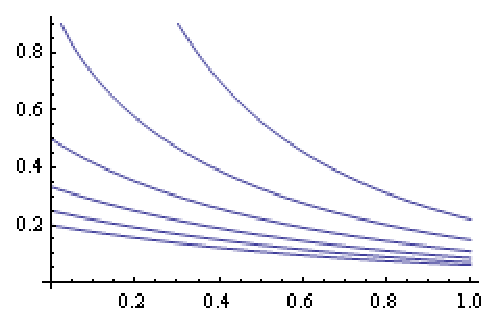
\includegraphics[width=0.4\textwidth]{economy/Ekintegral.eps}
	\end{center}
	\caption{Integration values for the Gamma function}
	\label{E2k}
\end{figure}

\subsection{Erlang prediction function}
The Erlang prior distribution is a Gamma prior with $k$ a chosen integer.
For example a $k=2$ gives:
\begin{equation}
 p(v_{final})\varpropto v_{final} e^{-v_{final}/\beta}
\end{equation}
The posterior distribution is:
\begin{eqnarray}
p(v) \varpropto \int^{\infty}_{v} e^{-v_{final}/\beta} dv_{final}\\
=-\beta e^{-v_{total}/\beta} \rvert^{\infty}_{v}\\
=\beta e^{-v_/\beta}
\end{eqnarray}
The posterior median is:
\begin{eqnarray}
P(v_{final}>v^*|v)=\int_{v^*}^{\infty} \frac{1}{\beta} e^{-(v_{final}-v)/\beta} dv_{final}\\
=e^{-(v^*-v)/\beta}
\end{eqnarray}
And we can find $v^*$ by imposing $e^{-(v^*-v)/\beta}=0.5$, thus obtaining a linear
 prediction function with unitary slope and intercept $\beta log2$:
\begin{equation}
 v^*=v+\beta log2
 \label{eq:ErlangPred}
\end{equation}
\subsection{Gaussian prediction function}
The Gaussian prior distribution:
\begin{equation}
 p(v_{final})\varpropto e^{-\frac{(v_{final}-\mu)^2}{2\sigma^2}}
\end{equation}
The posterior distribution of the Gaussian prior has no simple analytical form:

\begin{equation}
 p(v)\varpropto \int^{\infty}_{v} \frac{1}{v_{final}} e^{-\frac{(v_{final}-\mu)^2}{2\sigma^2}} dv_{final}
\end{equation}
Therefore to compute $p(v)$ we need to use a numerical integration method,
Fig.\ref{GaussianNumericalPosterior} shows the numerical integration results:

\begin{figure}[!htbp]
	\begin{center}
	\includegraphics[width=0.6\textwidth]{economy/GaussianPosterior2.eps}
	\end{center}
	\caption[Gaussian posterior distribution]{Gaussian posterior distribution computed via numerical integration.
	}
	\label{GaussianNumericalPosterior}
\end{figure}

The prediction function is also computed with numerical integration, plus optimisation.
Some prediction functions are shown in Fig.\ref{GaussianPredictions}.

\begin{figure}[!htbp]
	\begin{center}
	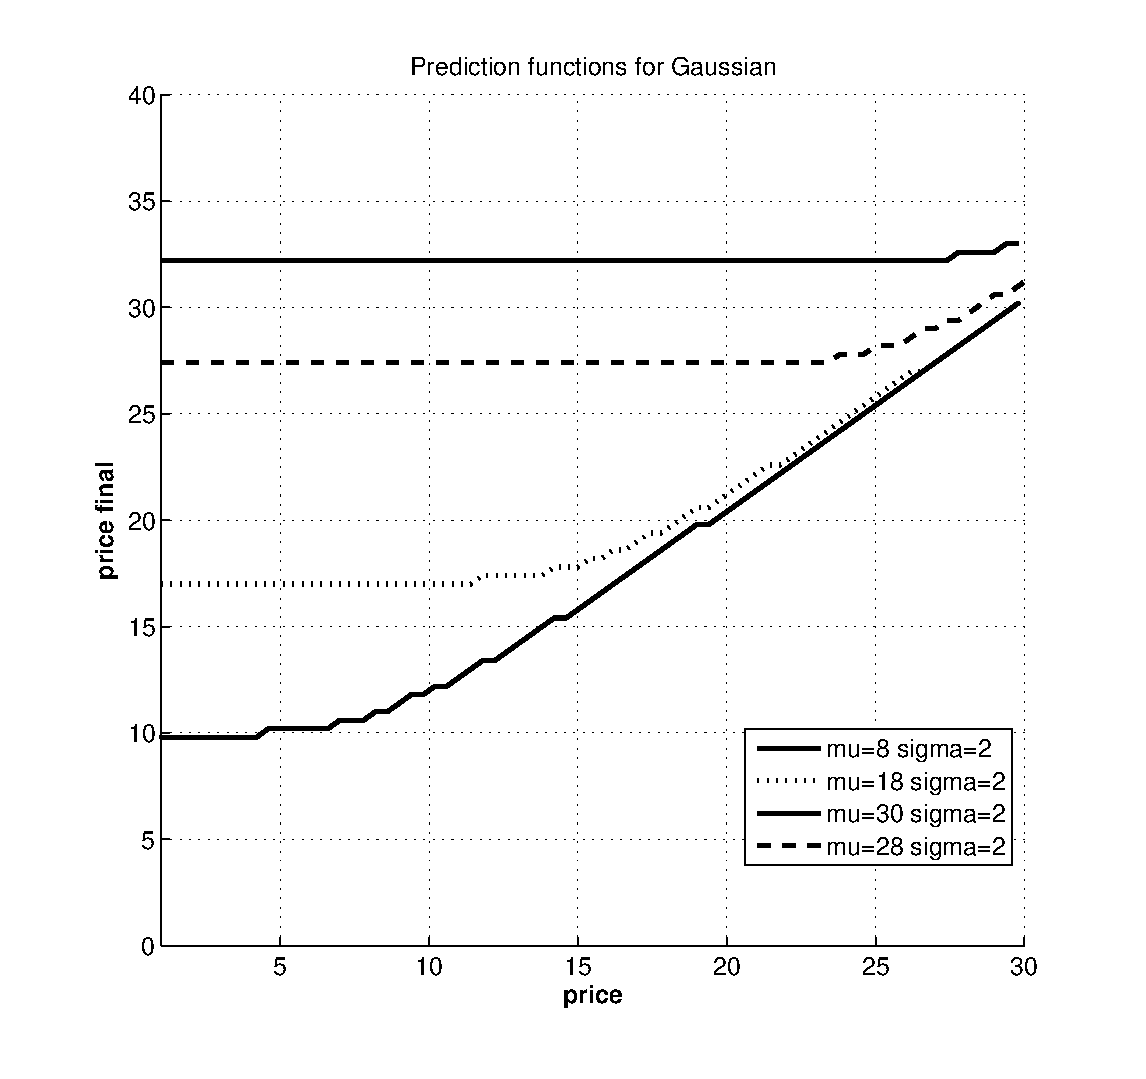
\includegraphics[width=0.6\textwidth]{economy/GaussianPredictors.eps}
	\end{center}
	\caption[Gaussian prediction function]{Gaussian predictions functions computed via numerical integration.
	}
	\label{GaussianPredictions}
\end{figure}

